Mutation testing is: <FIXME>.  Significant prior work, dating back to the
FIXMEs, aims to render mutation testing useful for constructing high quality
test suites and, by extension, software. 
Most of this previous mutation testing
research focuses on computing a mutation score, a measure of adequacy for a
given test suite.  However, this is computationally intensive for realistic
projects, because it requires requires running many tests on many modified
versions of a software system.  Reducing that computational cost is thus a major
thrust of mutation testing research~\cite{jia2011analysis}.   

Although test suite adequacy is certainly a useful thing to measure, the most
important goal of mutation testing\,---\,and indeed its original use
case~\cite{something}\,---\,is to help \emph{improve} a test suite.  For this
purpose, either a score or a list of all unkilled mutants generated across an
expensive mutation campaign is not useful for practicing engineers.  An
undifferentiated list of unkilled mutants contains many uninteresting or
redundant mutants, and a much smaller number of actionable mutants that are
maximally useful in guiding test improvement.  Thus, examining all unkilled
mutants is only practical for formal verification efforts or critical software
systems with high-powered test suites.  But even in these settings, examining
surviving mutants produced by modern mutation testing campaigns is
time-comsuming and unpleasant, as PI Groce and co-authors noted in prior work on
using mutants to drive formal verification and automated
testing~\cite{groce2015verified,groce2018verified,mutKernel}.


\begin{figure}
\centering
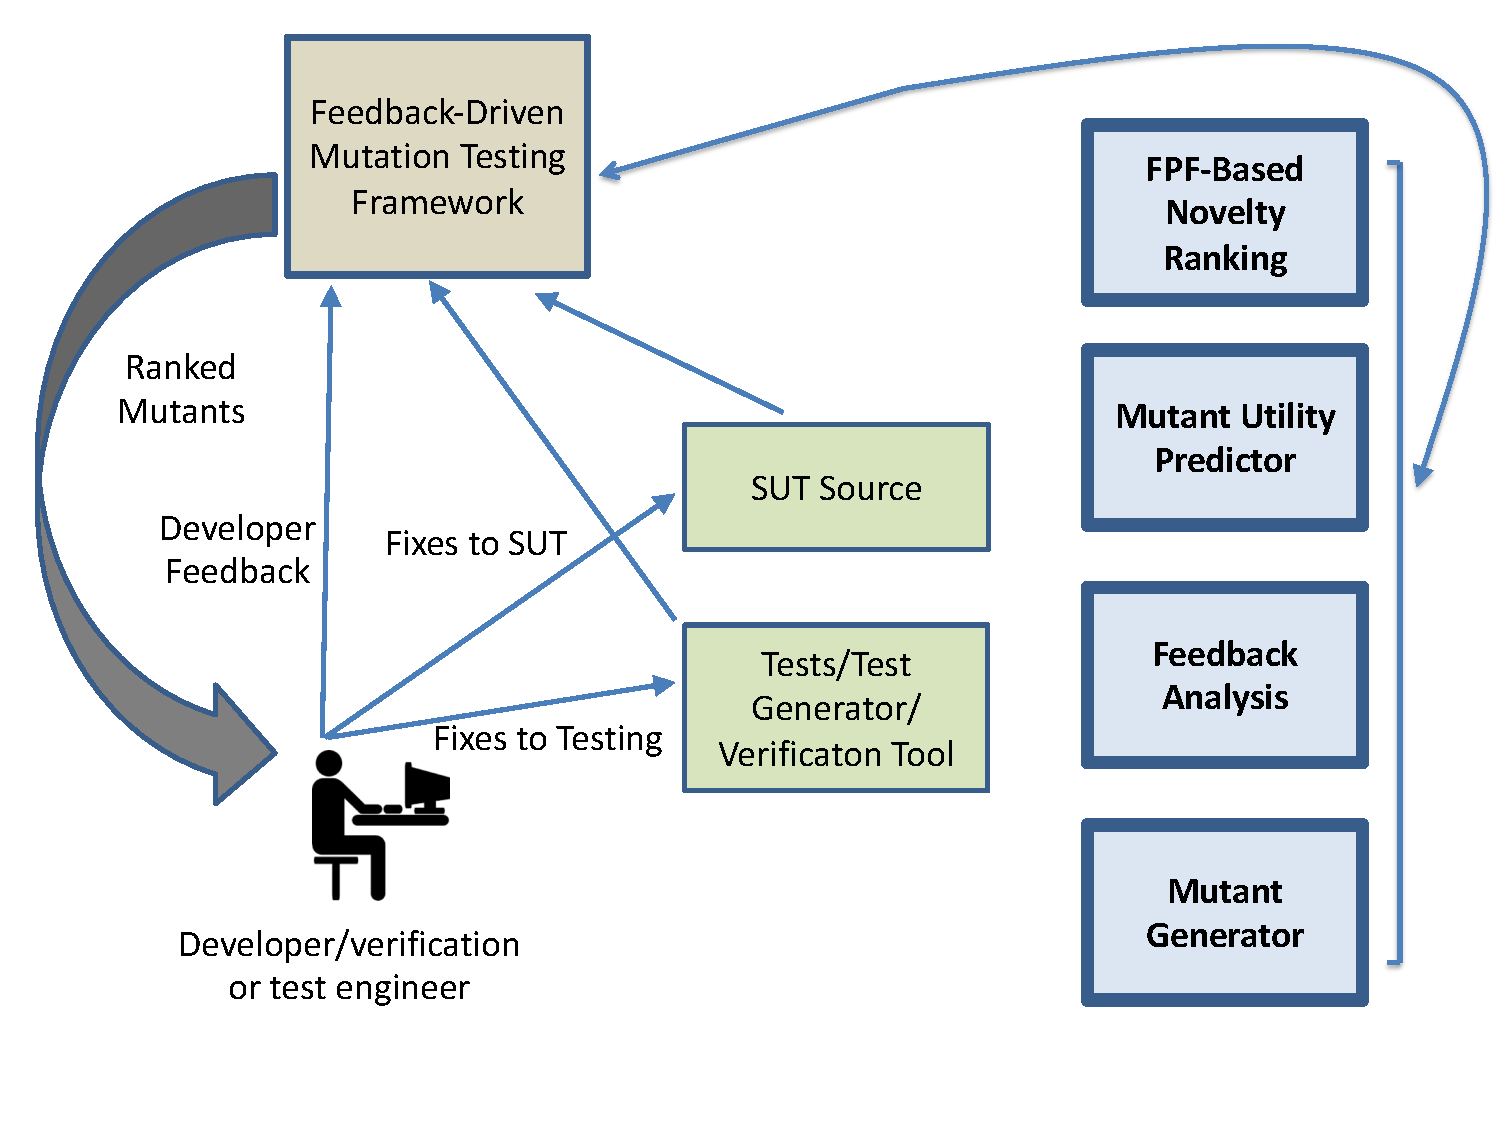
\includegraphics[width=0.8\columnwidth]{TestFlow}

\caption{Basic flow of feedback-driven mutation testing. FIXME: unify caption
  phrasing with ``just enough mutation testing'' while still talking about
  feedback-driven mutation.}
\label{fig:flow}
\end{figure}

Our goal is to enable \emph{Just Enough Mutation Testing}.  We propose a
mutation testing framework that identifies and presents a few, very different,
ranked mutants, and then works with the user to use those mutants to effectively
improve the program, the test suite, or both.  Figure~\ref{fig:flow}
 shows the basic outline of a proposed workflow
and components needed to support this agenda.  These components serve to
organize our research plan, which requires several fundamental novelties:
\begin{itemize}
\item \textbf{Efficient, any-language mutation testing.}  The most widely used
  mutation testing tool in the real world is PIT~\cite{pittest}, which targets
  Java bytecode.  There are recent attempts to provide the same kind of support
  for other languages, especially C, by targeting LLVM IR~\cite{HaririLLVM}.
  This poses several problems for real-world mutation testing.  First, bytecode-
  or IR-level mutation works well to compute a score for a test suite, but is
  not not suitable for presentation to developers or test engineers, who need to
  reason about a mutant's implications for their source or test code (i.e., Java
  developers think in terms of Java, not compiled bytecode).  Even when
  possible, translation may not help: a bytecode-level mutation may not have a
  simple source-level equivalent, especially if the bytecode has been optimized.
  Second, features that help identify semantically similar mutants are hard to
  identify at the bytecode level.  Even if the mutant is, for example, a
  constant replacement in one case and an arithmetic operator replacement in
  another, the fact that both take place inside an argument to a logging
  function with an {\tt INFO} argument may be enough to predict that their
  effects are redundant.  Finally, bytecode-level mutation is highly
  language-specific, leaving out popular languages like Python, Ruby, or Go, not
  to mention project-specific Domain Specific Languages (DSLs)~\cite{Fow10}.
  This is a problem for tool uptake and applicability: the vast majority of
  real-world software projects are written in multiple languages~\cite{Ray2014}.
  We propose novel mechanisms for \emph{efficient, any language mutation
    testing} based on our novel recent work on language-agnostic declarative
  program transformation using parser combinators~\cite{rvt-ppc}.  This
  technique operate at the source level and produces mutants and mutations that
  are easy for developers to understand. 
\item \textbf{Mutant prioritization and selection by predicted payoff.}
An unkilled mutant is, conceptually, very similar to a failing test.
With a larger number of unkilled
mutants, the problem becomes one very much like the bug triage or ``fuzzer
taming'' problem in random testing/fuzzing~\cite{PLDI13,SemCrash,semCrashBucketing}:  a user wants
to quickly find mutants that indicate the most important ``holes'' in a testing
or verification effort, and act on those most-critical gaps, possibly revealing
faults in the System Under Test (SUT). 
Fuzzers tend to produce very large numbers of failing tests for a much
smaller number of distinct bugs.  Finding the set of distinct bugs,
and identifying important bugs that need to be fixed immediately is
difficult, because the important bugs may be represented by only one
or two failing tests in a set of thousands of failing tests, most of
which are duplicates. 
Users do not (usually) care much
about finding the group of all tests failing due to a fault, or the
set of all mutants killable by the same extension to a test suite or
generator, but about seeing \emph{many very different test failures}
or \emph{many
  different unkilled mutants} quickly, to maximize the chance of
discovering the most important faults or holes in a testing effort.
However, current mutation testing approaches make
no real effort, with few exceptions~\cite{MutGoogle,FaRM} to prioritize mutants,
and none are based on a user-centered feedback loop, where the user and mutation
testing framework interact to improve a test suite, automated test generator, or
verification harness --- and the SUT.  Other than (arguably) some efforts to
incorporate dominance results~\cite{MutQuality}, no mutation testing approaches
currently suggest any more sophisticated way to maximize the novelty of
presented mutants than stratified sampling~\cite{gopinath2017mutation};
stratified sampling does not aim at semantic novelty, and can present many
mutants from the same class, if applied at the method level, even if those
mutants are highly similar in impact.  Other work~\cite{gopinath2015howhard}
proposes random sampling as the most effective way to select mutants.
Unfortunately, when an important class of unkilled mutants has only a few
members, random sampling is almost guaranteed to fail to present any of them.  
We propose to adapt clustering optimization techniques based on the idea of
novelty~\cite{Gonzalez85} to the problem of mutant selection, informed by a set
of novel diversity metrics selected for this domain. 
\item \textbf{User feedback elicitation and analysis.}
A
user's feedback about the most critical-to-test aspects of the code, or hard
work examining some mutants, has no influence on the kinds of sampling currently
proposed in the mutation testing literature.  
Even creating simple clusters of
mutants that are not killed due to the same underlying omission in tests
requires manual effort, with users, e.g., writing a Python script scanning
mutants for certain strings and assuming all mutated code with that string is
part of the same ``equivalence class.''  This is a tedious and error-prone
process, and only even possible once a ``kind'' of unkilled mutant is
discovered, largely by ad hoc scanning of the list of unkilled, uncategorized,
mutants.  
A constantly-updated ranking of mutants likely to be useful to examine
also helps provide a stopping rule other than patience, time available, or
``every last mutant'':  since mutants are ranked by likely payoff, once a user
has examined several mutants in a row without benefit, or mutants are highly
similar in behavior to other mutants, a user may reasonably stop, knowing that
the low-hanging fruit have probably all been picked.  Finally, a feedback-driven
mutation testing approach provides a new way to improve the efficiency of
mutation testing:  even for a very large project, it only has to build and
execute a small set of mutants, because it only runs the test suite on mutants
currently predicted to be of likely interest to the user.  
We propose ``feedback-driven'' mutation analysis that elicits and incorporates
user input on mutants, tests, and the SUT, supporting a concise, updating list
of mutants to inspect based on expected utility or payoff for the user.
\end{itemize}


\subsection{Problem Statement}

This project aims to make the use of program mutants practical in non-research settings, in a way that meets developers' actual needs: to make it possible for someone creating or enhancing a test suite to (1) use ``just enough'' mutation testing for their needs, maximizing benefit gained in exchange for work performed, and to (2) work in any programming language without worrying about the quality of tool support provided for mutation testing, and without sacrificing the ease of understanding of source-based mutants, while easily adding custom mutation operators that target their specific software development task.  This project also aims to make use of the insights of Test-Driven-Development (TDD), and proposes using mutation testing to move beyond a paradigm where developers build a series of tests narrowly tailored to steps in development, and use Mutation-Driven-Development (MDD) to build automated test generators or verification harnesses that handle not only anticipated problems imagined during development, but problems not anticipated by developers.  In addition to traditional manual testing, this proposal targets property-driven testing and full formal verification of software components, in order to be practical in the future, when software systems will often be so safety- or mission- critical that even ``good'' manual testing is simply not an acceptable approach.

\subsubsection{Just Enough Mutation Testing: Feedback-Driven Mutation Testing}


What a user really wants is a tool that presents a few, very different, ranked,
mutants, all likely to be of interest, and revises the presented mutants and
their ranking based on actions taken by the user --- adding tests, fixing
faults, marking certain mutants as equivalent or uninteresting, and perhaps
assigning a priority and severity to both killed or dismissed mutants and any
remaining un-handled mutants. 


Many mutants will be
pruned as part of an uninteresting category before they are ever executed, and
others will be omitted because they are ranked too low for the user to ever
consider. 

\begin{framed}
{\bf Problem:}  Develop highly automated methods and tools that allow the
practical application of mutation testing in a feedback-driven way, where user
and mutation testing framework cooperate to improve testing efforts, while
minimizing user effort and maximizing the ability to quickly find the most
important weaknesses of testing or verification. 
\end{framed}

\subsubsection{Any-Language Mutation Testing}

One ongoing limitation of mutation testing is that tools are often research
projects, and eventually become unusable due to lack of support, even in
mainstream languages such as Java and C~\cite{MutChoice}.

This is because mutation tools that parse a language and guarantee generation of
valid programs in the source language are complex, hard-to-maintain-and-extend
systems; language complexity makes such a tool for C++, for example, an
extremely daunting task.   

The problem with bytecode-level mutation is that while it

, and C and C+++ developers certainly do not generally understand LLVM IR; test
engineers are even less likely to appreciate such low-level descriptions.  

Even when possible, translation may not help: a bytecode-level mutation may not
have a source-level equivalent that is conceptually simple, especially if the
bytecode has been optimized, and some obvious source-level mutations (such as
statement deletion) are known to be difficult to implement in bytecode.
Moreover, targeting bytecode only helps with languages that compile to Java
bytecode or LLVM IR, which leaves out 

, and some obvious source-level mutations (such as
statement deletion) are known to be difficult to implement in bytecode.
Moreover, targeting bytecode only helps with languages that compile to Java
bytecode or LLVM IR, which leaves out 

  Finally, at the bytecode level, features that help identify mutants with similar semantic effects are obscured.  Even if the mutant is, for example, a constant replacement in one case and an arithmetic operator replacement in another, the fact that both take place inside an argument to a logging function with an {\tt INFO} argument may be enough to predict that their effects are redundant.

\begin{figure}
\begin{tabularx}{0.75\textwidth}{XXX}
\verb|\+ ==> -| & \verb|== ==> !=| & \verb|(\D)(\d+)(\D) ==> \1(\2+1)\3|\\
\verb|\+ ==> *| & \verb|== ==> <| & \verb|(\D)(\d+)(\D) ==> \1(\2-1)\3|\\
\verb|\+ ==> /| & \verb|== ==> >| & \verb|(\D)(\d+)(\D) ==> \g<1>0\3|\\
\verb|".+" ==> ""| & \verb|while ==> if| & \verb|(^\s*)(\S+.*)\n ==> \1\2\n\1break;\n|\\
%{\tt \\+ ==> *} & {\tt != ==> <=} & {\tt (\D)(\\d+)(\D) ==> \\1\\2-1\\3}\\
%{\tt \\+ ==> /} & {\tt != ==> >=} & {\tt ".+" ==> ""}\\
%{\tt \\+ ==> \%} & {\tt != ==> >=} & {\tt (^\\s*)(\\S+.*)\\n ==> \\1\\2\\n\\1break;\\n}\\
\end{tabularx}
\caption{Some universal mutation rules}
\label{fig:rules}
\end{figure}

PI Groce recently proposed~\cite{regexpMut} an approach to mutant generation that does not attempt to parse source code, but simply defines mutation operators by a set of regular-expression-defined text transformations.  These are organized into a hierarchy, so that if a program is, e.g., written in Swift, the ``universal'' mutation operators that apply to all programming languages are first applied, then operators for ``C-like'' languages, and finally a set of Swift-specific rules are applied.  Figure \ref{fig:rules} shows some of the current set of ``universal'' rules applied to all languages.  Adding a new language, even a custom DSL, or a new set of project-specific rules for an existing language, in this approach, simply requires writing a new rule file and defining where it lies in the language hierarchy.  In our feedback-driven setting, the problem of generating ``too many'' mutants is irrelevant: only a small set of highly diverse and likely-actionable mutants is ever presented to the user. %, and a novelty-estimator helps a user stop examining new mutants when the payoff is likely to be low.

There are significant limitations to this approach, however.  Because the source code is not parsed, and applies the regular expressions to lines of code, not larger blocks, the technique generates many mutants that are not valid programs, and cannot be compiled, or that are trivially equivalent because they, e.g., mutate ``source code'' in a large comment block.  Integrating mutation generation with execution is currently supported, but extending it to new languages or build systems is hard for users, requiring writing considerable Python code or complex shell scripts.  It is currently impossible to define mutation operators that apply to blocks of code rather than text within a single line, and standard regular expressions are not really suited to describing code constructs such as blocks, functions, classes, or structs.  Natural formatting of, e.g., an s-expression in a LISP-family language can hide opportunities for mutation, such as switching argument orders.  Finally, regular expressions are only occasionally a natural notation for expressing source-level mutation; source in all languages differs from arbitrary unstructured strings.

\begin{framed}
{\bf Problem:}  Provide high-quality user-friendly mutation generation methods to be used in a flexible but efficient mutation testing framework that can be applied to any source language, with support for easily adding custom operators or mutating DSLs.
\end{framed}

\subsubsection{Mutation-Driven-Development}

The primary focus of this project is to develop feedback-driven mutation testing.  However, the ideas of Test-Driven Development (TDD)~\cite{TDD,TDDFuture}, which repeatedly turns requirements into specific test cases, then implements just enough functionality to pass the current tests, can be generalized into a mutation-driven form.  A potential weakness (and, of course, an actual goal) of TDD is that the code will be narrowly tailored to the requirements, which produce the tests, which means that missing requirements will almost always be omitted both from the tests and the code.  For ``shall'' type behaviors~\cite{INCOSE}, this is not a key problem.  But for security and safety, ``shall not'' requirements that are omitted can be disastrous.  Mutation-Driven-Development (MDD) in its simplest form would require an application of feedback-driven mutation to the test suite at each development step, to ensure that code not only does what the tests require, but that the tests also sufficiently constrain the code to capture many implicit shall-nots.  Since such a process implemented by modifying TDD-driven tests would likely break the clean and appealing mapping between tests and requirements, and manual tests are inherently weak, for high-criticality systems, MDD should focus on augmenting TDD-driven tests with falsification-driven formal verification and automated testing.  One way to do this would be to ``elaborate'' TDD-produced unit tests into parameterized unit tests~\cite{UnitMeister,ParamUnit}, perhaps using a tool like DeepState~\cite{DeepState} for C/C++.  In such a process, weakness exposed by feedback-driven mutation testing would be addressed by taking an existing unit test and generalizing some parameters and assertions to kill the relevant mutants, letting AFL~\cite{aflfuzz}, libFuzzer~\cite{libfuzzer}, or a symbolic execution tool~\cite{angr1,angr2,manticore} identify specific inputs.  The focus of the MDD process would be on producing a test harness~\cite{WODACommon,tstlsttt} that allows an automated tool to kill interesting mutants.  More radically, MDD could be implemented via a radical departure from normal TDD, with a single testing or model checking harness iteratively enhanced with assertions and checks drawn from more requirements, always requiring the ability to kill (most) mutants of the current implementation.  This would not produce the usual large set of TDD tests, but instead produce a single high-powered test generator and formal specification.

\subsection{PI Qualifications}

PI Groce has been a user of, and contributor to, mutation testing tools for many years.  He combines a long research track record in software testing, including mutation testing, with actual experience testing critical software systems at NASA's Jet Propulsion Laboratory.  PI Groce's long-running interest in improving mutation testing arises from frustration in his efforts to apply mutation to the  Mars Science Laboratory's flight software, in particular to the file system~\cite{ICSEDiff,CFV08,AMAI}.  This practical orientation informs his recent work on using mutation testing in a falsification-driven approach to improving verification and automated testing efforts~\cite{groce2015verified,groce2018verified,mutKernel}.  PI Groce has extensive experience in developing mutation tools for new languages~\cite{le2014mucheck,muupi,regexpMut}, including the first reliable tools for mutation of Haskell, Python, and Swift, as well as in user-facing (vs. researcher-oriented) automated software testing tools~\cite{tstlsttt,DeepState}.  He additionally has expertise in driving testing of machine learning systems through user interaction~\cite{EndUserMistake,OnlyOracle}.

PI Le Goues is an expert in applied program analysis, program transformation,
and testing, most relevantly through her pioneering work in automated program
repair (both heuristic and semantic).  To this end, she has significant
experience with testing, mutation testing for fault localization and program
repair particularly, and the challenges of syntactic program modification. 
